\documentclass{rapportECL}
\usepackage{lipsum}
\usepackage{biblatex} %Imports biblatex package
\addbibresource{bibliotheque.bib}

\title{Rapport ECL - Template} %Titre du fichier

\begin{document}

%----------- Informations du rapport ---------

\titre{Un Langage "Pur" pour Web Assembly} %Titre du fichier .pdf
\UE{PSTL} %Nom de la UE

\enseignant{Frédéric \textsc{Peschanski}} %Nom de l'enseignant

\eleves{Lucas \textssc{Fumard} \\
	Lauryn \textsc{Pierre} \\
	Saïd Mohammad \textsc{ZUHAIR} } %Nom des élèves

%----------- Initialisation -------------------

\fairemarges %Afficher les marges
\fairepagedegarde %Créer la page de garde
\tabledematieres %Créer la table de matières

%------------ Corps du rapport ----------------
\section{Introduction}
Le but de notre projet est de concevoir un langage 100 $\%$ fonctionnel et “pur” pour WebAssembly en 
se basant sur cet article\cite{ullrich_counting_2020}(fourni). L'article défini un langage fonctionnel dont la gestion de la mémoire se fait par 
un mécanisme de comptage de références.
WebAssembly\cite{noauthor_webassembly_nodate} ou Wasm définit un format de code binaire portable
et un langage de type assembleur\cite{noauthor_webassembly_2023}. Tous les principaux navigateurs peuvent exécuter des programmes WebAssembly. 
Des langages comme C, C++, Rust, Go et bien d'autres peuvent être compilés en WebAssembly. 

\section{WebAssembly}

JavaScript est le seul langage de programmation native au Web. 
Pour de nombreuses raisons, JavaScript n’est pas idéal pour être une cible de compilation efficace pour les langages de bas niveau tels que C/C++ et Rust. 
WebAssembly a plusieurs objectifs\cite{haas_bringing_2017}. Être sûre, les programmes WebAssembly sont isolées de leur environnement hôte. 
WebAssembly est conçu pour être lié à aucun runtime ou langages de programmation, de sorte qu'il peut être exécuté sur n'importe quel 
appareil qui le prend en charge et d’avoir le même comportement. 
Ceci rend WebAssembly intéressant pour la création d'applications multiplateformes.
Les programmes pouvant être exécutées sur des ordinateurs de bureau, des appareils mobiles, et même des serveurs. 
WebAssembly fonctionne avec les technologies Web existants, telles que JavaScript, CSS, et HTML.
WebAssembly est un langage bytecode portable de bas niveau pris en charge par les principaux navigateurs Web. 
Les utilisations de WebAssembly ne se limitent pas qu'au domaine du Web, il y a aussi un intérêt pour l'Internet des Objets, les serveurs, les systèmes embarqués.
\par WebAssembly a un format texte (.wat) et un format binaire (.wasm). 
WebAssembly peut être exécuté dans différents environnements, tels que les serveurs, les navigateurs web ou les applications. 
Dans les navigateurs web, WebAssembly est exécuté en même temps que le code JavaScript. 
Pour les serveurs, WebAssembly est exécuté en utilisant des runtimes tels que Node.js. 
Plusieurs compilateurs ont été développés pour WebAssembly\cite{noauthor_wabt_2023,noauthor_wasm3_2023,noauthor_wasmer_nodate,noauthor_wasmtime_nodate}. 
Wasmer\cite{noauthor_wasmer_nodate} et wasmtime\cite{noauthor_wasmtime_nodate} sont les plus connus. 
Ils utilisent tous les deux la technique de la compilation à la volée. Wasmtime est développé en collaboration supervisée par la fondation Mozilla. 
Alors que wasmer est développé par une entreprise privée. 
Dans le cadre de notre projet, on utilise wabt\cite{noauthor_wabt_2023} pour compiler et on exécute le compilé à l’aide de Node.js\cite{noauthor_nodejs_nodate}. 
\par Les programmes sont composés d'un ou plusieurs modules. Un module contient la définition des fonctions, variables globales. 
Les définitions peuvent être importées ou exportées.
Ils interagissent avec l’environnement à l’aide d’import et d’export explicites. 
Un module doit être validé avant l’exécution pour s’assurer qu’il est bien typé et sûr d’exécuter. 
WebAssembly possède un système de type statique centré autour de quatre valeurs :  i32, i64, f32 et f64. 
Ces types désignent respectivement les entier sur 32 bit, les entiers sur 64 bits, les nombres flottants sur 32 bits et les nombres 
flottants sur 64 bits.
La spécification officielle de Wasm comprend une sémantique formelle pour le langage, 
avec une déclaration précise de la propriété de solidité des types prévue. 
Elle a d'abord été publiée dans un premier projet en 2017, puis dans la norme officielle, appelée WebAssembly 1.0 (Wasm 1.0), en 2019.
\par La mémoire d’un programme Wasm repose sur le modèle de mémoire linéaire\cite{haas_bringing_2017}. 
La mémoire linéaire est un tampon continu d'octets non signés  que JavaScript et Wasm peuvent lire et modifier de manière synchrone. 
Au cours de l’exécution, l’espace mémoire peut grandir. 

\begin{figure}[ht]
	\centering
	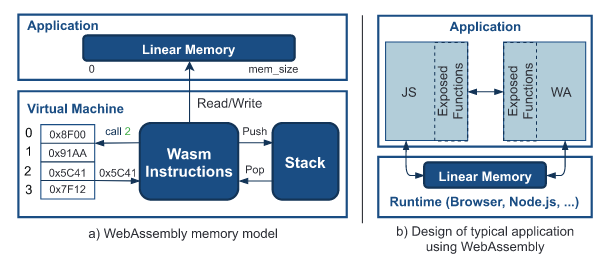
\includegraphics[scale=0.55]{logos/model_memory_wasm.png}	
	\caption{WebAssembly Architecture \cite{noauthor_wasmati_nodate}}
\end{figure}
\FloatBarrier 



\section{Lecture de l'article} \label{section:article}
Le langage fonctionnel décrit dans l'article\cite{ullrich_counting_2020} alloue ses constructeurs dans la pile et manipule des 
adresses vers ces emplacements mémoire alloués. Il est donc primordial d'avoir un système d'allocation et réutilisation de 
mémoire performant afin d'éviter les fuites mémoires et un temps d'exécution faible.

Le système de la gestion de la mémoire par comptage de référence est bien plus vieux que des systèmes par garbage collector, 
mais aussi plus efficaces\cite{ullrich_counting_2020}. Cependant, la gestion de mémoire comptage de références ne fonctionne que si 
il n'est pas possible de créer de cycle de référence. 
C'est pourquoi les garbage collector sont plus utilisés de nos jours.

Les auteurs de l'article\cite{ullrich_counting_2020} ont créé un langage fonctionnel dans lequel les cycles de références 
sont impossibles afin d'implémenter un système de gestion de mémoire par comptage de référence et d'obtenir un langage fonctionnel 
dont l'exécution est optimisée. Ils définissent un langage source $\lambda_{pure}$. 
Qui, après une étape de compilation, deviendra $\lambda_{RC}$, notre langage de destination.
$\lambda_{RC}$ est une extension de $\lambda_{pure}$ auquel on a ajouté les instructions de gestion de la mémoire : 
\verb|inc|, \verb|dec|, \verb|reset|, \verb|reuse|.
Notre interpréteur implémentera le langage $\lambda_{pure}$ et notre compilateur, le langage $\lambda_{RC}$.


Les tâches que nous avons identifiées sont les suivantes :

\begin{itemize}
	\item Analyser le fonctionnement de WASM et étudier son écosystème
	\item Programmer un parseur qui puisse lire le langage pur tel que défini dans l'article\cite{ullrich_counting_2020}
	\item Programmer un interpréteur en Rust du langage selon les sémantiques du langage pur
	\item Définir quelques tests unitaires couvrant les sémantiques définies dans l'article
	\item Ajouter la gestion des instructions \verb|inc|, \verb|dec|, \verb|reset|, \verb|reuse|
	\item Programmer un compilateur du langage agrandi vers WASM
\end{itemize}

Comme dans l'article, nous partons du principe que le typage a déjà été vérifié et que les \verb|let| inutiles ont été enlevés.

\section{AST}

Concernant la grammaire du langage, nous reprenons celle qui est définie dans la section 3 de l'article et retranscrit dans la Figure ~\ref{fig:grammaire pure} ci-dessous.

\begin{figure}[hbt!]
	\centering
	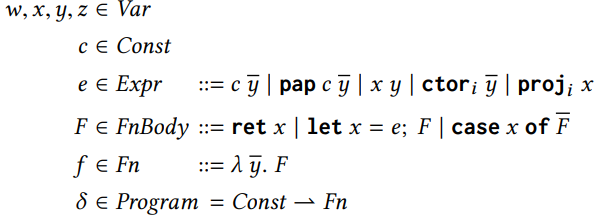
\includegraphics[scale=0.70]{logos/grammaire.png}
	\caption{Grammaire du langage source $\lambda_{pure}$}
	\label{fig:grammaire pure}
\end{figure}
\FloatBarrier

Nous avons implémenté en Rust l'AST du langage proposé par les auteurs, en en étendant les 
expressions (\verb|Expr|) pour ajouter la notion d'entiers à notre interpréteur,
afin de tester concrètement notre interpréteur à partir de fichiers de programmes.

Chaque type dans l'AST est un produit de somme en Rust. Nous utilisons principalement les entier 32 bits, les chaînes de caractères,
ainsi que les vecteurs (ou tableaux), notés respectivements \verb|i32|, \verb|String| et \verb|Vec| en Rust.

\bigskip

Les énumérateurs feuilles dans notre AST sont les variables \verb|Var| et les constantes \verb|Const|,
qui contiennent chacune une chaîne de caractère décrivant le nom de la fonction pour les constantes et 
le nom de la variable pour les variables. La valeur de la variable peut être récupérée dans le tas
une fois que l'on a l'adresse, obtenue à partir de la pile et de la chaîne de caractère.

\medskip

Une expression peut être un appel de fonction (\verb|FnCall(Const, Vec<Var>)|), un appel de fonction partielle (\verb|PapCall(Var, Var)|),
une fonction partielle (\verb|Pap(Const, Vec<Var>)|), un constructeur (\verb|Ctor(i32, Vec<Var>)|), 
l'obtention d'un champ d'un objet (\verb|Proj(i32, Var)|), ou un entier (\verb|Num(i32)|).

\medskip

Chaque constructeur est défini par un entier différent, détaillé par les constantes globales ci-dessous.

\begin{figure}[H]
\begin{equation*}
CONST\_FALSE = 0
\end{equation*}
\begin{equation*}
CONST\_TRUE = 1
\end{equation*}
\begin{equation*}
CONST\_NIL = 2
\end{equation*}
\begin{equation*}
CONST\_LIST = 3
\end{equation*}
\begin{equation*}
CONST\_NUM = 4
\end{equation*}
\caption{Type des constructeurs dans le langage $\lambda{pure}$}
\label{listing:types_ctor}
\end{figure}
\FloatBarrier 
Ainsi, nous avons défini les booléens \verb|False| et \verb|True| par les entiers \verb|0| et \verb|1| respectivement.

Nous utilisons des identifiants plutôt qu'une somme de produit où l'on pourrait définir chaque type proprement car 
c'est de cette façon que nous allons stocker les types en mémoire en WASM.

Une fois le contructeur créé, nous pouvons accéder aux champs du contructeur avec l'instrution \verb|proj|.
Il est à noter que seules les listes ont des champs, car ce sont les seuls constructeurs qui prennent
des variables en paramètres pour être créés.

\medskip

Une application partielle \verb|Pap| est un appel de fonction dans lequel il manque des arguments, 
et un appel de fonction partiel \verb|PapCall| est une application partielle désignée par une variable
à laquelle nous ajoutons une autre variable, augmentant le nombre d'arguments d'un. 
Une fois qu'il y a assez d'arguments dans le vecteur d'arguments de l'application partielle,
la fonction désignée est exécutée, avec tous les arguments.

\bigskip

En remontant dans l'AST, nous trouvons les corps de fonction qui peuvent être le retour de fonction d'une variable \verb|Ret(Var)|, 
une affectation de variable \verb|Let(Var, Expr, FnBody)| ou un match du type d'une variable 
\verb|Case(Var, Vec<FnBody>)|.

\medskip

L'affectation interprète son expression afin d'injecter la valeur en résultant dans le tas, donc l'adresse est associée
au nom de sa variable, sur la pile. Ainsi, cette variable référencera la valeur de l'expression
dans la suite de la fonction.

\medskip

Pour savoir quelle branche du \verb|Case| il faut exécuter, il suffit tout simplement de regarder
l'identifiant du type du constructeur puis accéder à l'indice correspondant dans le vecteur des branches du \verb|Case|. 
Ainsi, si l'on veut exécuter du code pour les listes, il faut d'abord remplir les branches de \verb|False|, 
\verb|True| et \verb|Nil|. Il n'est pas nécessaire de remplir la branche pour les entiers si on considère qu'aucun entier
ne sera jamais évalué dans ce \verb|Case|. Le cas échéant, l'interprète lance une erreur et le comportement
du langage compilé en WASM est indéterminé.

\medskip

Le corps de fonction à la racine de la fonction, encapsulant tous les corps suivant, 
est lui-même encapsulé dans la définition d'une fonction \verb|Fn| composée d'une liste (un vecteur en Rust) de variables \verb|Vec<Var>| ainsi que
d'un corps de fonction \verb|FnBody|.

\medskip

Enfin, à la racine de notre AST, nous définissons un \verb|Program| en Rust comme une table de hachage liant des constantes \verb|Const| à 
des définitions de fonction \verb|Fn|.

\bigskip

\section{Parser/reader}

Notre reader utilise la bibliothèque Chumsky\cite{zesterer_chumsky_nodate}, ainsi, nous ne pouvons pas stoker les noms définis 
variables, ce qui nous empêche de distinguer directement les constantes des variables, car sans historique de définition de variable, 
tous les mots en paramètres de fonction sont interprétés commes des constantes.

C'est pourquoi nous avons besoin de transformer certaines constantes et certains appels de fonctions en variables et applications partielles à l'aide de 
fonction d'explorations définies dans le fichier \verb|transform_var.rs|.
Les variables définies avec un \verb|let| sont donc ainsi représentées par \verb|Var| au lieu de \verb|Const| dans l'AST à interpréter,
et les applications non complètes en applications partielles

Nous ajoutons par ailleur un préfixe "var\_" aux variables définies par l'utilisateur.

Ainsi, nous avons obtenu un AST bien formé et correct, où une constante est réellement une constante et une application
complète est aussi réellement une application complète.

\section{Interpréteur}

La première étape de notre projet était de créer un interpréteur du langage $\lambda{pure}$, sans instruction de gestion de références.

\subsection{Mémoire}

Afin d'implémenter un interpréteur du langage décrit, il nous a d'abord fallu implémenter les structures permettant d'accéder à la mémoire, dont les structures du tas et de la pile (\verb|Heap| et \verb|Ctxt|), comme définies par les auteurs de l'article selon la Figure ~\ref{fig:memory} ci-dessous.

\begin{figure}[hbt!]
	\centering
	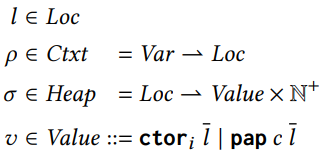
\includegraphics[scale=0.80]{logos/figure_strutures_interpreteur.png}
	\caption{Structures de gestion de la mémoire} 
	\label{fig:memory}
\end{figure}
\FloatBarrier 


\verb|Loc| est l'adresse de la case mémoire allouée pour la valeur dans le tas. C'est la valeur de retour de toutes les sémantiques 
du langage, tel que définies dans la figure 1 de l'article\cite{ullrich_counting_2020}.
Contrairement à l'article, nous avons choisi de ne pas retourner un nouveau tas à chaque fois, mais de garder un même tas que 
l'on modifie par effet de bord.


\subsubsection{Pile et tas}

La pile est une structure de type FILO liant une variable \verb|Var| à une adresse \verb|Loc| que nous étendons à chaque définition de variable. Nous passons la pile étendue à le suite du programme, sans la transmettre à l'appelant. Ainsi, la pile est automatiquement dépilée lorsque l'on quitte le block d'affectation de variable.

Le tas \verb|Heap| est une structure contenant le nombre total d'allocations ainsi qu'une table de hachage d'un entier vers un \verb|Value|, où \verb|Value| est définie comme soit un constructeur, soit un entier.
Pour la compilation, nous allons réserver la première case pour stocker le nombre d'allocations totales, ainsi, cette case est définie à 1 dans un tas vide.

Ces structure nous permettent donc de lier une variable à sa valeur dans la mémoire. Nous ajouterons les références dans la compilation.

%La pile est implémentée par un énumérateur \verb|Ctxt| contenant les champs pour le nom de la variable, l'emplacement de la variable dans le tas, ainsi que la suite de la pile. 
%On agrandit cette pile en l'englobant dans un nouvel énumérateur \verb|Ctxt| contenant les champs de la nouvelle variable ainsi que l'ancienne pile. 

%Nous ne transmettons pas la pile crée à l'appelant, ainsi la pile est automatiquement dépilée lorsque l'on quitte le block d'affectation de variable.

%Pour chercher une variable, nous parcourons la pile de l'extérieur vers l'intérieur de façon récursive jusqu'à obtenir la variable souhaitée ou arriver à la fin de la pile, dans quel cas l'interpréteur produit une erreur.

%Ainsi, nous obtenons une structure de type FILO caractérisant le comportement d'une pile.

%Nous avons choisi de diverger un peu de l'article\cite{ullrich_counting_2020} en introduisant un tas changé par effet de bord, et non passé en sortie de block afin de rendre une seule valeur de retour.

%Ce tas \verb|Heap| est une structure contenant le nombre total d'allocations ainsi qu'une table de hachage d'un entier vers un \verb|Value|, où \verb|Value| est définie comme soit un constructeur, soit un entier.
%Pour la compilation, nous allons réserver la première case pour stocker le nombre d'allocations totales, ainsi, cette case est définie à 1 dans un tas vide.

%Cette structure permet de lier des emplacements et les valeurs et fonctionne avec \verb|Ctxt|. 

%Les auteurs de l'article stockent un couple \verb|(Valeur, entier)|, où l'entier est le nombre de références de l'objet. Nous l'implémentons dans le compilateur, mais comme l'interpréteur n'adapte que la partie pure du langage, le nombre de références n'est jamais modifié. De ce fait, nous avons préféré enlever la présence de ce nombre dans l'interpréteur pour simplifier la lecture du code.

%Ainsi, \verb|Ctxt| permet de prendre une référence associée à un nom de variable et \verb|Heap| permet de prendre la valeur associée à cette référence.


\subsection{Interprétation}

Une fois le programme parsé et transformé, nous pouvons interpréter le programme, c'est-à-dire exécuter une expression dans le 
contexte du programme. Toutes les fonctions de l'interpréteur s'exécutent avec une pile et un tas. Ainsi, nous créons une pile vierge
et un tas vide que nous passons en référence à chaque fonction de l'interpréteur.

Ensuite, il nous suffit d'interpréter les instructions en respectant les règles sémantiques du langage telles que définies à la figure 1, section 4 de l'article\cite{ullrich_counting_2020}.
%selon la Figure ~\ref{fig:semantics} ci-dessous.

%\begin{figure}[hbt!]
%	\centering
%	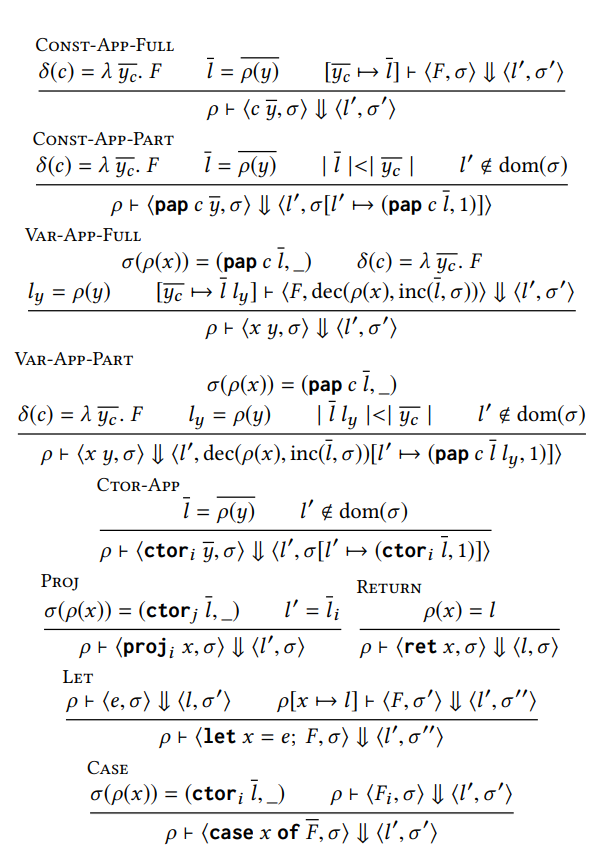
\includegraphics[scale=0.80]{logos/semantics.png}
%	\caption{Sémantiques du langage $\lambda_{pure}$}
%	\label{fig:semantics}
%\end{figure}
%\FloatBarrier 


\medskip


Il est à noter que, comme indiqué précédemment, nous ne renvoyons pas le nouveau tas à chaque instruction, comme les auteurs, 
mais seulement l'emplacement de l'objet dans la mémoire, car nous avons préféré modifier le tas par effet de bord.

Nous n'avons pas non plus implémenté les instructions \verb|inc|, \verb|dec|, \verb|reset|, et \verb|reuse|, et donc la notion de références dans cet interpréteur car ces instructions ne font pas partie du langage $\lambda_{pure}$, mais du $\lambda_{RC}$.
Nous les implémentons donc dans le compilateur, qui compile le langage $\lambda_{RC}$ étendu.

Ainsi, hormis le tas et l'apparition des instructions \verb|inc| et \verb|dec|, nous avons strictement respecté les règles sémantiques du langage $\lambda_{pure}$ défini par les auteurs de l'article.

\medskip

Ainsi, pour interpréter un \verb|let|, nous interprétons d'abord l'expression associée et nous étendons la pile avec l'adresse de la valeur de l'expression interprétée. Nous passons cette nouvelle pile dans la suite du programme.

%Ainsi, pour interpréter un \verb|let|, nous interprétons d'abord l'expression associée, qui renvoie un emplacement dans le tas de la valeur interprétée, et nous lions cet emplacement à la variable du \verb|let| en étendant la pile, qui nous passons dans la suite du programme.

%Pour un \verb|case|, il suffit de récupérer le type de la valeur dans le tas de dont l'emplacement a été lié dans la pile à la variable donnée, puis interpréter la suite de l'AST stocké dans un vecteur selon le type du constructeur (voir Figure~\ref{listing:types_ctor}).
Pour interpréter un \verb|case|, nous récupérons le type de la variable par la pile puis le tas.
Une fois le type de la variable récupéré, il s'agit d'un simple accès à un vecteur.

Pour interpréter un \verb|proj|, nous récupérons la liste des arguments du constructeur par la pile puis le tas. Il suffit ensuite de renvoyer le bon champ, si tenté qu'il existe.

%Pour un \verb|proj|, nous récupérons la valeur à travers la pile puis le tas, puis, si l'index du champ demandé ne dépasse pas la taille du vecteur des champs du constructeur, nous renvoyons l'emplacement stocké.

Pour l'application complète, nous fixons les arguments donnés aux paramètres de la fonctions dans une nouvelle pile et nous interprétons le corps de cette fonction avec cette pile.

%Pour l'interprétation des applications de constantes, il faut d'abord savoir s'il s'agit d'une primitive ou d'une fonction définie par l'utilisateur, puis nous fixons les arguments aux noms des paramètres de la fonction, puis nous exécutons le corps de la fonction.
%Il n'y a pas besoin de vérifier que le nombre d'arguments soit exact, car le transformateur s'est occupé de transformer celles-ci en définitions d'applications partielles sur des constantes.

Enfin, s'il s'agit d'une application partielle, si l'argument ajoutée permet d'exécuter l'appel, nous l'interprétons comme une application complète. Sinon, nous copions l'ancienne application partielle et ajoutons l'argument à la liste des arguments.
%Enfin, s'il s'agit d'une application partielle, nous vérifions le nombre d'arguments, puis nous exécutons une routine similaire, en interprétant le corps de la fonction demandée avec les arguments fixés si le nombre d'arguments correspond, ou nous renvoyons une nouvelle application partielle étendue du nouvel argument appliqué s'il n'y en a pas assez.

\bigskip

Nous avons par ailleurs défini un certain nombre de primitives arithmétiques et booléennes qui nous permettent d'écrire et 
de tester des programmes dans le langage $\lambda_{pure}$.

\begin{figure}[H]
	\begin{itemize}
		\item Fonctions arithmétiques (\verb|add|, \verb|sub|, \verb|mul|, \verb|div|, \verb|mod|)
		\item Fonctions booléennes sur booléens (\verb|and|, \verb|or|, \verb|not|)
		\item Fonctions booléennes sur nombres (\verb|eq|, \verb|sup|, \verb|inf|, \verb|sup_eq|, \verb|inf_eq|)
	\end{itemize}
	\label{primitives}
	\caption{Liste des primitives implémentées}
\end{figure}

\bigskip

Nous avons testé cet interpréteur en créant plusieurs tests sur les sémantiques, mais aussi quelques programmes simples, 
tels que le calcul de fibonacci dont voici l'implémentation dans le langage.
%, ou le programme \verb|swap| défini à la page 5 de l'article\cite{ullrich_counting_2020}.

\begin{figure}[H]
	\begin{lstlisting}
  fibo n = let m = 1;
    let a = inf_eq n m; case a of
    (   let m1 = 1;
        let x = sub n m1; let f1 = fibo x;
        let m2 = 2;
        let y = sub n m2; let f2 = fibo y;
        let r = add f1 f2; ret r)
    (ret n)
	\end{lstlisting}
	\caption{Implémentation d'un algorithme naïf de calcul de fibonacci}
	\label{listing:fibo_naif}
\end{figure}
\FloatBarrier 

\section{Compilateur}

La dernière étape de notre projet est de créer un compilateur du langage $\lambda{RC}$. Pour cela, il faut insérer les 
instructions \verb|inc|, \verb|dec|, \verb|reset| et \verb|reuse| dans l'AST. 

Ainsi, la première chose à faire est
d'étendre l'AST et de créer un transformateur du langage $\lambda{pure}$ vers le langage $\lambda{RC}$.

\subsection{AST}

Nous étendons donc l'AST du langage $\lambda{pure}$ en suivant l'extension faite par les auteurs de l'article\cite{ullrich_counting_2020},
selon la figure~\ref{fig:grammaire RC}.

\begin{figure}[hbt!]
	\centering
	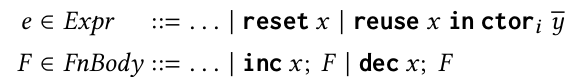
\includegraphics[scale=0.40]{logos/grammaire_RC.png}
	\caption{Extension de la grammaire du langage $\lambda_{RC}$}
	\label{fig:grammaire RC}
\end{figure}
\FloatBarrier 

\subsection{Insertion des instructions de références} \label{section:insert_inc_dec}

Cette section correspond à la section 5 de l'article \cite{ullrich_counting_2020}.
L'insertion des instructions \verb|inc|, \verb|dec|, \verb|reset| et \verb|reuse| se fera en trois étapes :
\begin{enumerate}
    \item Insérer \verb|reset| et \verb|reuse|
    \item Inférer les paramètres des fonctions
    \item Insérer \verb|inc| et \verb|dec|
\end{enumerate}

\subsubsection{Insertion de reset et reuse}
En utilisant ces deux instructions, on peut réduire la quantité de mémoire allouée et libérée en réutilisant les cellules mémoire lorsque les valeurs ne sont pas partagées. Cela permet d'économiser des ressources et d'optimiser les performances en évitant des opérations coûteuses d'allocation et de libération de mémoire.

Les deux instructions \verb|reset| et \verb|reuse| sont utilisées ensemble. Si $x$ est une valeur partagée, alors $y$ est initialisée avec une référence spéciale, et l'instruction reuse alloue simplement une nouvelle valeur de constructeur \verb|ctor|. 
Si $x$ n'est pas partagé, alors reset décrémente les compteurs de références des composants de $x$, et $y$ est initialisée à $x$. 
Ensuite, reuse réutilise la cellule mémoire utilisée par x pour stocker la valeur d'un constructeur \verb|ctor|. Pour savoir si x est une variable partagée, on vérifie son compteur de références.

On introduit la fonction $\delta_{reuse}$ qui se charge d'insérer les instructions \verb|inc| et \verb|dec| dans une fonction. Pour cela, elle fait appel à la fonction \textit{R} sur le corps de la fonction.
En plus de la fonction \textit{R}, on utilise deux autres fonctions : \textit{D} et \textit{S}.
Pour chaque case, \textit{R} tente d'insérer des instructions \verb|reset|\textbackslash \verb|reuse| pour la variable correspondant au case. Cela est fait en utilisant \textit{D} dans chaque bras du case.
La fonction \textit{D} cherche les variables mortes. Elle prend en paramètre la variable $z$ à réutiliser et l'arité $n$ du constructeur correspondant. 
\textit{D} recherche le premier emplacement où $z$ où n'est pas utilisée dans le reste du corps de la fonction, puis fait appel à \textit{S} en lui donnant une nouvelle variable. 
Dans notre implémentation, nous gardons un compteur qu'on incrémente à chaque fois qu'on a besoin d'une nouvelle variable. Et on passe à \textit{S} une variable de la forme $w\_compteur$. Pour s'assurer qu'on utilise toujours une nouvelle variable, on interdit le fait qu'une variable puisse avoir un nom de la forme $w\_nombre$. Si aucune instruction \verb|ctor| correspondante ne peut être trouvée, \textit{D} ne modifie pas le corps de la fonction. Sinon, on insère un \verb|reuse|.
La fonction \textit{S} réalise les substitutions. \textit{S} prend en argument une variable, une arité et une partie du corps de la fonction. Si S trouve un constructeur dont l'arité est n. \textit{S} remplace ce constructeur par \verb|reuse|.


\subsubsection{Inférence}
Dans cette partie, on veut créer une map $\beta$ qui associe à chaque fonction une liste qui donne le status des paramètres : "Owned" ou "Borrowed".
On va s'appuyer sur la fonction \textit{collect\_O} qui retourne un ensemble contenant les variables qui doivent être "owned".
Un paramètre est "owned" si une de ses projections est "owned" ou s'il est passé en argument à une fonction qui prend un paramètre "owned".
Si une variable x est utilisé dans un \verb|reset|, on ne veut pas qu'elle soit "borrowed". 
En effet, on utilise le compteur de référence pour savoir si une variable est partagé lors de l'évaluation d'un \verb|reset|. 
Or si x est "borrowed", il peut être une variable partagé et son compteur à un.
De plus, une application ne doit pas avoir de paramètre borrowed. Pour résoudre ce problème, on définit une enveloppe $c_O := c$. 
Dans notre implémentation, le nom de $c_O$ est de la forme $nom de la fonction$\_c. 
Pour s'assurer que que la constante $c_O$ n'est pas présente dans le programme, interdit au nom de fonction d'avoir pour suffixe \_c.
Chaque \verb|pap| c y est remplacé par \verb|pap| $c_O$ y. On ajoute à $\beta$ une entrée tel que $\beta(c_O) = \overline{O}$

La fonction $\delta_{\beta}$ va déduire la valeur de $\beta$ pour une fonction c. 
Pour réaliser cette étape, on commence par une approximation $\beta(c)$ = $\overline{B}$ , puis en calculant $S = collect\_O(b)$. 
Ensuite, nous mettons à jour  $\beta(c)_i :=$ O  si $y_i \in S $, et nous répétons ce processus jusqu'à atteindre un point fixe où aucune autre mise à jour 
n'est effectuée sur $\beta(c)$.
Pour inférer l'ensemble du programme, on appelle $\delta_{\beta}$ sur chaque fonction dans l'ordre de déclaration des fonctions. 
Si une fonction $c$ utilise une autre fonction $d$, pour avoir avoir un résultat optimal, il faut que $d$ soit déclarée avant $c$. 
Sinon, on considère que les paramètres de la fonction $d$ sont "owned".


\subsubsection{Insertion de inc et dec}
Dans cette partie, on insère les instructions \verb|inc| et \verb|dec|.
Lorsqu'une variable est borrowed, elle ne possède pas la responsabilité de sa gestion mémoire. 
D'un autre côté, une variable "owned" est responsable de sa gestion mémoire.
Les compteurs des variables doivent être incrémentées avant d'être utilisées dans un contexte "owned". 
Si elle est utilisée dans un constructeur ou dans une application.
On doit décrémenter leur compteur de référence das variables "owned" après leur dernière utilisation. 
On suppose que notre map $\beta$ de la section précédente est bien définie. 
Pour chaque fonction c, on introduit une nouvelle map $\beta_l$ qui associe à chaque variable dans c, son statut ('B' ou 'O'). 
$\beta_l$ est initialisé avec les valeurs de $\beta(c)$. Par défaut, une variable sera considérée comme owned.

Nous définisson plusieurs fonctions :
\begin{itemize}
    \item $O_x^{+}$: la variable x n'est pas incrémentée si elle est "owned" et morte.
    \item $C$ : appelée sur le corps de la fonction pour effectuer l'ajout d'instruction \verb|inc| et \verb|dec|.
    \item $C_{app}$: se charge des applications en effectuant des appels récursifs sur les paramètres et leur statut.
    \item $O^{-}$: sert à décrémenter plusieurs variables, utilisée au début d'un case et d'une fonction.
    \item  $O_x^{-}$: décrémente la variable x si elle est "owned" et morte.   
\end{itemize}

% Si on a un tail call pour le préserver, on change  $\beta(c)_i$ = O si c est utilisé dans le tail call et $\beta_l(x_i)$ est owned.

\subsection{Environnement d'exécution}

Notre compilateur génère du code sous le format WAT, le format texte du langage WebAssembly. Ainsi, nous avons besoin
du compilateur \verb|wat2wasm| pour créer du code WASM compilé.

Pour être exécuté, un module WASM a besoin d'être appelé par un script JavaScript. Ainsi, nous avons créé un fichier \verb|runtime.js| qui regroupe toutes les fonctions nécessaires à l'exécution d'un module WASM ainsi que l'interprétation du résultat obtenu. Nous avons aussi ajouté des fonctions de création de constructeurs de façon à créer et à ajouter des objets dans la mémoire avant d'appeler une fonction du module WASM.

\subsection{Structure de la mémoire en WASM}

Pour implémenter le langage $\lambda{RC}$ en WASM, nous avons besoin de deux structures essentielles : le tas et la pile.

La pile n'a pas besoin que nous implémentons une de structure particulière, car nous utilisons la pile de WASM lors de l'appel d'une fonction (le cadre de la fonction).

\medskip

Afin d'implémenter le tas en WebAssembly, nous utilisons une structure \verb|Memory| qui nous permet de définir une mémoire que nous pouvons manipuler de WebAssembly ainsi que de JavaScript.
C'est dans cette mémoire que nous stockons les objets que nous créons.
L'accès à cette mémoire nous permettra de réaliser des diagnostics ainsi que des évaluations de l'empreinte mémoire.
La case mémoire 0 est réservée pour indiquer le prochain espace mémoire libre. Par défault, nous mettons la valeur de cette case à 
l'adresse de la seconde case, soit 4, car la mémoire est alignée sur des entiers naturels de 32 bit ou 4 octets.
Ensuite, chaque constructeur défini dans la figure~\ref{listing:types_ctor} suit le format suivant : \verb|<type> <nb_ref> <args>|. 

Les argument des types prennent une case mémoire chacun, c'est à dire la place d'un entier signé 32 bits. 
%Il est certain qu'il s'agit d'un gachi de place de donner 4 octets pour chaque argument, mais WebAssembly n'a pas de type plus petit, et, bien que l'on puisse lire et stocker des entiers sur 16 ou 8 bits,
%cela complexifierait le déboguage de l'implémentation que d'utiliser 32 bits pour représenter plusieurs arguments.
Ainsi, l'alignement de la mémoire sera toujours de 32 bits, soit 4 octets. Les adresses de nos variables seront toujours 
multiples de 4.

Nous ordonnons donc les objets dans la mémoire selon la figure~\ref{listing:memory_wasm} suivante.

\begin{figure}[H]
	\begin{itemize}
		\item False : 0 <\#refs>
		\item True  : 1 <\#refs>
		\item Nil   : 2 <\#refs>
		\item List  : 3 <\#refs> <@arg1> <@arg2>
		\item Num   : 4 <\#refs> <entier>
	\end{itemize}
	\caption{Schéma mémoire des constructeurs}
	\label{listing:memory_wasm}
\end{figure}

Ainsi, un constructeur \verb|FALSE| référencé deux fois est représenté sous la forme "\verb|0 2|" dans la mémoire et un entier 10 
référencé 3 fois sous la forme "\verb|4 3 10|".

\bigskip

Nous avons aussi décidé de stocker les applications partielles dans le tas de la même façon que toutes les autres valeurs.
Il nous faut cependant trouver une alternative au stockage du nom de la fonction en une chaîne de caractères, car WebAssembly ne supporte pas ce type. 
Ainsi, nous avons décidé de donner à chaque fonction, primitive ou définie par l'utilisateur, un identifiant sous forme d'un entier, qui nous servira à choisir quelle fonction appeler lors de l'exécution de l'application partielle.
%Il nous faut aussi définir un nouveau nombre définissant le type des applications partielles, étendant les types déjà définis par à la Figure~\ref{listing:types_ctor}. 
%Bien que nous définissions les applications partielles de la même façon que les constructeurs, les applications partielles n'en sont pas. 
Nous ajoutons un nouveau type pour les applications partielles à notre liste des types de la figure~\ref{listing:types_ctor}.


\begin{figure}[H]
	\begin{equation*}
	CONST\_PAP = 5
	\end{equation*}
	\caption{Type des PAP en WASM}
	\label{listing:types_pap_wasm}
	\end{figure}
	\FloatBarrier 

Ainsi, dans la mémoire, nos applications partielles sont stockés sous la forme de la figure~\ref{listing:memory_wasm_pap} suivante.

\begin{figure}[H]
	\begin{itemize}
		\item Pap   : 5 <\#refs> <id fonction> <\#arguments fixés> <@arg1> <@arg2> ...
	\end{itemize}
	\caption{Schéma mémoire pour les applications partielles}
	\label{listing:memory_wasm_pap}
\end{figure}

Par exemple, une application partielle est sous la forme \verb|5 1 7 2 12 14 0| où \verb|5| est le type "application partielle", 
\verb|1| est le nombre de références à cette application partielle, 
\verb|7| est l'identifiant de la fonction à appeler (dans l'interpréteur, on utilise des \verb|string|), 
\verb|2| est le nombre d'arguments fixés et \verb|12| et \verb|14| sont les arguments fixés et
\verb|0| est l'emplacement des arguments non fixés que la fonction peut accepter.

\subsection{Compilation des instructions en WAT}

Il nous faut compiler les instructions du langage $\lambda{pure}$ ainsi que les nouvelles instructions \verb|inc|, 
\verb|dec|, \verb|reset| et \verb|reuse|. Pour ces nouvelles instructions, nous suivons les sémantiques définies par les auteurs, 
définies à la figure 2 dans la section 5.1 de l'article\cite{ullrich_counting_2020}.

%Il nous faut compiler les instructions du langage $\lambda{pure}$ dont nous avons les sémantiques sur la figure~\ref{fig:semantics}
%ainsi que les nouvelles instructions \verb|inc|, \verb|dec|, \verb|reset| et \verb|reuse|. Pour ces nouvelles instructions, nous
%suivons les sémantiques définies par les auteurs présentes dans la figure~\ref{fig:semantics_rc} ci-dessous.

%\begin{figure}[hbt!]
%	\centering
%	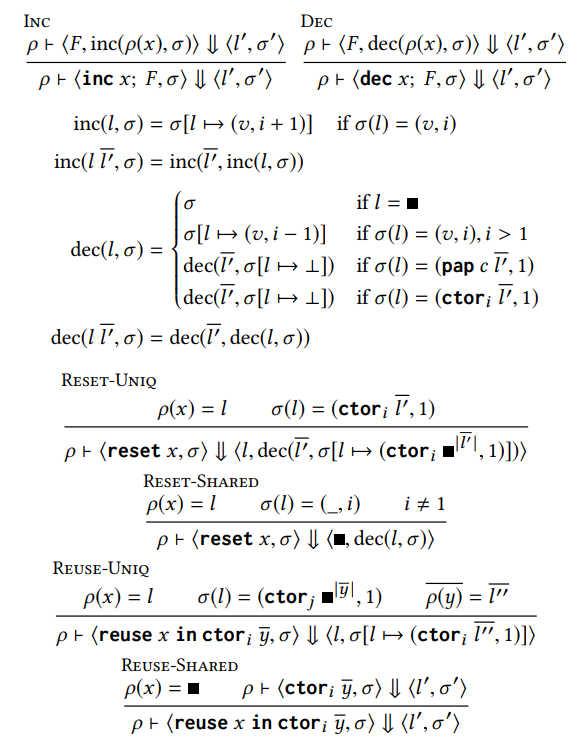
\includegraphics[scale=0.80]{logos/semantics_rc.png}
%	\caption{Sémantiques de la partie $\lambda_{RC}$ du langage}
%	\label{fig:semantics_rc}
%\end{figure}
%\FloatBarrier 
WebAssembly est un langage possédant des fonctions où il est possible d'écrire dans un style fonctionnel, avec les instructions 
imbriquées les unes dans les autres, entrourées de parenthèses, ou impératif, une instruction par ligne.
Nous avons choisi d'adopter un style impératif dans la compilation des instructions de WebAssembly car ce style nous permet 
de regrouper des instructions récurentes en fonctions, ce qui simplifie la lecture du code du compilateur. Cependant, nous utilisons
quelques fois dans la compilation et dans ce rapport le style fonctionnel.
Ces deux styles sont strictement égaux et valides en WebAssembly.

\subsubsection{Formation des objets dans la mémoire}

Pour créer les objets dans la mémoire, nous avons écrit quelques fonctions en WebAssembly.
Ces fonctions, \verb|__make_num|, \verb|__make_no_arg|, \verb|__make_list| et \verb|__make_pap|, modifient la mémoire
pour y former un objet du type demandé. Puis, ces fonctions modifient l'emplacement 0 de la mémoire, pour y écrire le
prochain emplacement libre, aligné sur 4 octets. 

Chaque fonction implémente dans la mémoire un des quatre stockages différents définis dans le schéma de la 
mémoire à la figure~\ref{listing:memory_wasm}.

\medskip

%\bigskip

%La fonction la plus simple est \verb|__make_no_arg|. C'est avec cette fonction que nous créons des objets sans paramètres, soit les booléens \verb|False| et \verb|True| et le mot de fin de liste \verb|Nil|. Pour utiliser cette fonction, nous chargeons d'abord l'identifiant du type demandé, soit \verb|CONST_FALSE| (0), \verb|CONST_TRUE| (1) ou \verb|CONST_NIL| (2), puis \verb|__make_no_arg| met cet identifiant à l'adresse désignée par la case 0, initialise le nombre de références à 1 dans la case d'adresse suivante, et incrémente de 8 la valeur de la case 0 pour l'aligner à la prochaine case vide. 
%Enfin, l'adresse de l'objet créé est renvoyée.

%Ainsi, l'objet est créé et la prochaine adresse disponible est définie comme étant celle de la case suivant l'objet.

%\bigskip

%Les fonctions \verb|__make_num| et \verb|__make_list| ont un fonctionnement similaire, mais prennent en paramètres non pas le l'objet, mais les arguments de l'objet à créer, soit l'entier à créer pour \verb|__make_num|, et les adresses des objets composant la tête et la queue de la liste pour \verb|__make_list|. La valeur de la case 0 est incrémentée de 12 et de 16 respectivement.

%\bigskip

%Enfin, la fonction \verb|__make_pap| prend seulement l'identifiant de la fonction appliquée. Elle écrit ensuite le type de l'objet, soit \verb|CONST_PAP| (5), le nombre de références (1), l'identifiant de la fonction donné en paramètre et le nombre d'arguments fixés, initialisé à 0. La fonction libère ensuite la place nécessaire à l'écriture de l'ensemble des arguments fixés.
%Elle incrémente donc la valeur de la case 0 de $16 + N * 4 $ où $N$ est le nombre d'arguments que la fonction de l'identifiant attend.
\medskip
Nous avons aussi défini la fonction inter \verb|$__nb_args|, qui est compilée de sorte à associer chaque identifiant de fonction au nombre de paramètres, que nous récoltons au préalable à la compilation, avec l'utilisation des instructions \verb|block| et \verb|br_table|.

L'utilisation de ces deux instructions est la suivante.

\begin{figure}[H]
	\begin{lstlisting}[escapeinside={(*@}{@*)}]
  (block $b1
    (block $b2
      local.get $x (*@ \label{ex_br_table_x}@*)
      (br_table $b2 $b1)
    ) (*@ \label{ex_br_table_b2}@*)
    i32.const 0 (*@ \label{ex_br_table_0}@*)
    return
  ) (*@ \label{ex_br_table_b1}@*)
  i32.const 1 (*@ \label{ex_br_table_1}@*)
  return
	\end{lstlisting}
	\caption{Exemple d'utilisation de block et br\_table en WebAssembly}
	\label{listing:example_block_br_table}
\end{figure}

Des \verb|block|s avec un label \verb|$l| peuvent être définis. L'on peut sortir du \verb|block| en enbranchant au label du \verb|block| avec une instruction du type \verb|br $l|.

La \verb|br_table| est une table permettant d'effectuer un embranchement selon la valeur en haut de la pile.
La valeur 0 embranchera sur la branche d'index 0, la valeur 1 embranchera sur la branche d'index 1, etc.
Il est à noter qu'une valeur supérieure à la taille de la table embranchera sur la dernière branche de la table.

Ainsi, en associant les deux, et avec la figure~\ref{listing:example_block_br_table} comme exemple, si la valeur x (ligne~\ref{ex_br_table_x}) est \verb|0|, la table embranchera à la fin du block \verb|$b2| pour exécuter la suite du programme (ligne~\ref{ex_br_table_b2}) et retourner la valeur \verb|0|. Si la valeur de x (ligne~\ref{ex_br_table_x}) est \verb|1| ou supérieure, la table enbranchera à la fin du block \verb|$b1| pour exécuter la suite du programme (ligne~\ref{ex_br_table_b1}) et retourner la valeur \verb|1|.

Ces deux instructions de WebAssembly seront aussi utiles pour la compilation de notre instruction \verb|case|.

\subsubsection{Compilation des fonctions}

Pour compiler une fonction, il faut d'abord récolter le nom de toutes les variables utilisées afin de les 
déclarer et on y ajoute une variable utile à certains scenarios de compilation, \verb|$__intern_var|.
Ensuite, nous changeons le nom interne de la fonction pour ajouter "fun\_" devant pour éviter les 
redéfinitions de fonctions internes.
Nous avons également ajouté "var\_" à toutes les variables définies grâce au transformateur.
Cela nous permet de définir des variables internes telles que \verb|__intern_var| qui ne peuvent pas être modifiées par 
l'utilisateur.

Puis, on compile le corps de la fonction, et on ajoute derrière une parenthèse fermante pour fermer la fonction.

Ainsi, la structure de la fonction \verb|fibo| de la figure~\ref{listing:fibo_naif} est la suivante :
\begin{figure}[H]
	\begin{lstlisting}[escapeinside={(*@}{@*)}]
  (func $fun_fibo (export "fibo") (param $n i32) (result i32)
    (local $__intern_var i32)
    (local $var_m1 i32)
    (local $var_m2 i32)
    (local $var_a i32)
    (local $var_r i32)
    (local $var_y i32)
    (local $var_x i32)
    (local $var_m i32)
    ;; corps de la fonction
  )
	\end{lstlisting}
	\caption{Compilation de la signature de la fonction fibo}
	\label{listing:signature_fibo}
\end{figure}

\subsubsection{Let}

Le \verb|let| est très simple à compiler, en effet, il faut compiler l'expression en premier pour mettre la valeur de retour 
dans la variable, et compiler le reste de la fonction. Pour une variable \verb|x| définie par l'utilisateur, le code est donc le suivant

\begin{figure}[H]
	\begin{lstlisting}[escapeinside={(*@}{@*)}]
  ;; expression
  local.set var_x
  ;; corps de fonction suivant
	\end{lstlisting}
	\caption{Compilation d'un let}
	\label{listing:compile_let}
\end{figure}


\subsubsection{Case}

Pour compiler les \verb|case|, nous avons besoin d'une structure nous permettant d'exécuter une branche du code suivant la valeur du 
type de la variable donnée. Ainsi, nous utilisons la combinaison de \verb|block| et \verb|br_table| aussi utilisée pour l'exécution
d'une application partielle, comme montré sur la figure~\ref{listing:example_block_br_table}.

Le code d'une instruction \verb|case| à deux embranchements sur la variable \verb|x| définie par l'utilisateur 
se compile ainsi de la manière suivante


\begin{figure}[H]
	\begin{lstlisting}[escapeinside={(*@}{@*)}]
  (block $__case0
    (block $__case1
      local.get $var_x
      i32.load
      (br_table $_case1 $_case0)
	)
    ;; suite si type False
  )
  ;; suite si type True
	\end{lstlisting}
	\caption{Compilation d'un case}
	\label{listing:compile_case}
\end{figure}

\subsubsection{Proj}

On ne peut exécuter un proj que sur un objet de type \verb|CONST_LIST|, car c'est le seul constructeur qui contient des champs qui
pointent vers d'autres objets.

Pour compiler un $proj_i$, il suffit donc de renvoyer le champ désigné par i, soit ajouter $(i + 1)*4$ à l'adresse de la variable, car
d'après notre schéma de la mémoire, le seul constructeur possédant des champs est la liste, dont les champs commencent deux cases 
après le début de l'objet.
Il ne faut pas oublier que nous commençons l'indexation des champs à 1, c'est-à-dire que $proj_1$ donne le premier champ, 
$proj_2$ le deuxième, etc.

Ainsi, pour une variable \verb|x| de type liste définie par l'utilisateur, la compilation de $proj_1$ est la suivante.
\begin{figure}[H]
	\begin{lstlisting}[escapeinside={(*@}{@*)}]
  local.get $var_x
  ;; calcul de l'offset en ajoutant la case des references et sur alignement des entier 32 bits
  i32.const 8 ;; (i + 1) * 4
  i32.add     ;; calcul de l'adresse a recuperer
  i32.load    ;; chargement du champ (adresse d'un objet)
\end{lstlisting}
\caption{Compilation d'un $proj_1$}
\label{listing:compile_proj}
\end{figure}

\subsubsection{Application complète}

Pour l'application complète d'une fonction définie par l'utilisateur, il faut charger tous les arguments donnés puis appeler 
l'équivalent de la fonction en compilé. Ainsi, l'application des variables \verb|x| et \verb|y| définiées par l'utilisateur sur 
la fonction \verb|f| définie par l'utilisateur se compile selon la figure~\ref{listing:compile_app_comp_const}.

\begin{figure}[H]
	\begin{lstlisting}[escapeinside={(*@}{@*)}]
  local.get $var_x
  local.get $var_y
  call $fun_f
	\end{lstlisting}
	\caption{Compilation d'une application complète}
	\label{listing:compile_app_comp_const}
\end{figure}

Si la fonction est une primitive, nous appliquons les arguments sur la définition de la primitive en WebAssembly.
Voici par exemple dans la figure~\ref{listing:compile_add} la compilation de la primitive \verb|add| appliquée aux variables 
\verb|x| et \verb|y| définies par l'utilisateur.

\begin{figure}[H]
	\begin{lstlisting}[escapeinside={(*@}{@*)}]
  ;; decallage de deux entiers, la place de la valeur du nombre
  (i32.load (i32.add (local.get $var_x) (i32.const 8)))
  (i32.load (i32.add (local.get $var_y) (i32.const 8)))
  i32.add
  call $__make_num
  
  (call $__dec (local.get $var_x))
  (call $__dec (local.get $var_y))
	\end{lstlisting}
	\caption{Compilation d'une application sur une primitive}
	\label{listing:compile_add}
\end{figure}

Il ne faut pas oublier de décrémenter les références des objet, car leur des \verb|inc| ont été ajoutés, comme spécifié dans la 
section~\ref{call $__dec$} lors de l'application sur \verb|add| dans l'expression \verb|add x y|.

\subsubsection{Application partielle}

L'application d'une variable sur une application partielle est délicat. En effet, nous avons choisi d'implémenter les applications partielles en stockant toutes les variables appliquées dans la mémoire. Cependant, cela signifie que nous devons copier l'application partielle avant d'y fixer la nouvelle variable et incrémenter le nombre d'arguments. Nous appelons donc la fonction \verb|__copy_pap| qui crée une nouvelle application partielle du même type et copie les arguments un à un. Il ne faut pas oublier de decrémenter les références de l'application partielle copiée.

Puis, s'il y a assez de variables fixées d'après \verb|__nb_args|, nous appelons la fonction \verb|__exec_pap|, qui charge les variables une à une sur la pile d'exécution de WebAssembly avec une \verb|loop| puis nous appelons la fonction ou nous compilons la primitive selon l'identifiant de la fonction de l'application partielle. Enfin, nous déréférençons l'application partielle.

De la même manière qu'avec la compilation de \verb|case|, nous savons quelle branche appeler grâce à la combinaison des instructions \verb|block| et \verb|br_table|. Une fois le code compilé, cette fonction est assez longue, car elle contient toutes les primitives définies ainsi que tous les appels des fonctions définies par l'utilisateur.

\subsubsection{Inc et dec}

La compilation d'un \verb|inc| est très simple. En effet, nous ajoutons \verb|1| au nombre de références de l'objet. 
Ainsi, pour une variable \verb|x| définie par l'utilisateur, le code compilé est le suivant.

\begin{figure}[H]
	\begin{lstlisting}[escapeinside={(*@}{@*)}]
  ;; chargement de l'adresse pour le stockage
  local.get $var_x

  ;; chargement des references
  (i32.add (local.get $var_x) (i32.const 4))
  i32.load
   
  ;; calcul des nouvelles references
  i32.const 1
  i32.add

  ;; stockage
  call $__set_ref

  ;; corps de fonction suivant
	\end{lstlisting}
	\caption{Compilation d'un inc}
	\label{listing:compile_inc}
\end{figure}

Avec la fonction interne \verb|__set_ref| permettant de fixer le nombre de références.

%\begin{figure}[H]
%	\begin{lstlisting}[escapeinside={(*@}{@*)}]
%  (func $__set_ref (param $adr i32) (param $ref i32)
%    ;; mise a jour des refs
%    local.get $adr ;; @x
%    i32.const 4    ;; @x 4
%    i32.add        ;; @refs
%    local.get $ref ;; @refs #refs
%    i32.store      ;;
%  )
%	\end{lstlisting}
%	\caption{Fonction \_\_set\_ref}
%	\label{listing:set_ref}
%\end{figure}

Le \verb|dec| est un peu plus compliqué, car il ne suffit pas seulement de décrémenter le nombre de références, il faut aussi appliquer un \verb|dec| sur les arguments des \verb|ctor| et \verb|pap| lorsque ceux-ci se retrouvent à 0.
Ainsi, nous définissons une fonction \verb|$__dec|, qui décrémente l'objet et les arguments de l'objet si besoin.

La fonction \verb|__dec| décrémente donc les références de l'objet de façon similaire à \verb|inc|, en utilisant \verb|i32.sub| au lieu de \verb|i32.add|, puis si ce nombre de références est nul, teste le type de l'objet. Si ce type est celui de \verb|CONST_LIST|, on charge le premier champ de l'objet, pour y appliquer la fonction \verb|$__dec| et de même sur le deuxième champ. Si le type est ceui de \verb|CONST_PAP|, on utilise une boucle (\verb|loop $nom_boucle| en WebAssembly) pour charger et chacun des objets du \verb|pap| et y appliquer la fonction \verb|$__dec|.

\subsubsection{Reset et reuse}

La fonction \verb|__reset| décrémente le nombre de références de la variable donnée et renvoie \verb|0| si la variable est effectivement détruite ou l'adresse de la variable si elle est encore en vie. Voici le code WebAssembly de cette fonction.

\begin{figure}[H]
	\begin{lstlisting}[escapeinside={(*@}{@*)}]
  (func $__reset (param $var_var i32) (result i32)
    (call $__dec (local.get $var_var))
    (i32.add (local.get $var_var) (i32.const 4))
    i32.load
    i32.eqz
    if
      i32.const 0
      return
    end
    local.get $var_var
  )
	\end{lstlisting}
	\caption{La fonction reset}
	\label{listing:compile_reset}
\end{figure}

Il suffit ensuite de charger la variable concernée et d'appeler cette fonction \verb|__reset|.

\medskip

L'instruction \verb|reset| est toujours suivie d'une instruction \verb|reuse|. Celle-ci teste si l'adresse de la variable donnée, 
soit le résultat de l'instruction \verb|reset|, nul puis s'il y a assez de place dans l'ancienne variable. Si le résultat de ces
tests est \verb|1|, on peut copier les arguments donnés après \verb|reuse| dans l'emplacement mémoire de l'ancienne variable.

Sinon, on doit créer un nouvel objet selon le \verb|ctor| donné.

\section{Résultats}

Noous avons testé notre interpréteur et notre compilateur sur la fonction de fibonacci naïf telle que définie sur la figure~\ref{listing:fibo_naif}.

\begin{table}[H]
	\begin{tabular}{|c|r|r|r|r|r|}
	\hline
	\textbf{n} &
		\multicolumn{1}{c|}{\textbf{fibo(n)}} &
		\multicolumn{1}{c|}{\textbf{\begin{tabular}[c]{@{}c@{}}Temps\\ exécution\\ interprété\end{tabular}}} &
		\multicolumn{1}{c|}{\textbf{\begin{tabular}[c]{@{}c@{}}Temps\\ exécution\\ compilé\end{tabular}}} &
		\multicolumn{1}{c|}{\textbf{\begin{tabular}[c]{@{}c@{}}Total allocations\\ mémoire\\ (interprété et compilé)\end{tabular}}} &
		\multicolumn{1}{c|}{\textbf{\begin{tabular}[c]{@{}c@{}}Objets\\ en vie\\ compilé\end{tabular}}} \\ \hline
	5  & 5       & 0 ms     & 0.015 ms  & 66         & 1 \\ \hline
	10 & 55      & 10 ms    & 0.095 ms  & 795        & 1 \\ \hline
	15 & 610     & 153 ms   & 0.562 ms  & 8 877      & 1 \\ \hline
	20 & 6 765   & 2.18 s   & 3.77 ms   & 98 508     & 1 \\ \hline
	25 & 75 025  & 30.2 s   & 34.17 ms  & 1 092 531  & 1 \\ \hline
	30 & 832 040 & 6.5 mins & 366.94 ms & 12 116 415 & 1 \\ \hline
	\end{tabular}	
	\caption{Résultats de l'exécution de fibo sur l'interprète et en compilé}
	\label{table:results}
\end{table}

En testant notre interpréteur et notre compilateur sur une implémentation de la fonction de fibonacci (voir Figure~\ref{listing:fibo_naif}), nous obtenons les bons résultats de ficonacci, avec un temps d'exécution et un nombre total d'allocations dans la mémoire qui augmentent ded façon exponentielle.

Nous remarquons que les instructions \verb|reset|, \verb|reuse| n'ont pas été insérées dans ce code, car il y a autant d'allocations pour le code interprété que pour le code compilé. Nous remarquons également que nous obtenons à chaque fois un seul objet en vie à la fin de l'exécution du code compilé, c'est à dire un seul objet dont le nombre de références n'est pas nul. 

Ainsi, les instructions \verb|inc| mais surtout \verb|dec| ont bien été insérées avec succès dans le code pour modifier le nombre de références des objets au fur et à mesure de l'exécution.

\section{Améliorations possibles}

Comme précisé à la fin de la section~\ref{section:article}, nous avons implémenté un compilateur en partant du principe que le 
typage est bon et que les \verb|let| inutiles ont été enlevés. Le langage implémenté n'est donc pas typé statiquement.

De plus, nous avons implémenté les applications partielles de la façon la plus simple à laquelle nous avons pensé. 
Cette implémentation n'est pas optimale car nous créons une nouvelle application partielle avant de l'exécuter et de la détruire.

Nous aurions pu utiliser un unique objet global pour des constructeurs sans arguments tels que $False$, $True$ ou $Nil$. 
Nous avons en effet choisi de créer des objets à chaque fois pour avoir plus d'éléments sur lesquels agir. Dans une 
version plus complète du compilateur, il serait plus intelligent de rendre ces constructeurs sans arguments uniques. L'on 
pourrait par ailleur introduire une meilleure gestion de la mémoire semblable à un \verb|malloc| en C. De plus, on peut 
utiliser un i32 pour représenter les types et le nombre de références, avec les instructions \verb|i32.store16_u| et \verb|i32.load16_u|, qui stockent et chargent des entiers sur 16 bits non signés.

Quand on infére les status des paramètres d'une fonction, nous parcourons les fonctions dans l'ordre de leur déclarations. 
Si jamais une fonction c utilise une autre fonction $d$ avant qu'elle soit déclaré on considère ses paramètres comme étant "owned".
On peut changer notre implémentation, pour inférer $d$ au lieu de lui supposer que ses paramètres sont "owned".
Bien sûr nous devrions mettre en place un mécanisme pour les fonctions mutuellement récursives.

%De plus, nous n'avons pas non plus implémenté la récursion terminale en WebAssembly. Cependant, l'optimisation des \verb|dec| et \verb|inc| sur une récursion terminale dans la section~\ref{section:insert_inc_dec} est tout de même utile.

\newpage

\printbibliography
\end{document}
